\chapter{Estado del Arte\label{sec:estado_del_arte}}

[Quizá convenga en este apartado comenzar enfocando el problema a la captación del movimiento en general y despues pasar, al tema de la rehabilitación de manos]

Dada la importancia de la capacidad de capturar el movimiento de las manos cada vez son más los proyectos basados en este eje central.\\
-esto no encaja bien aquí  \\
Desde el estudio de la manera de estudiar el movimiento de cualquier parte del cuerpo de los humanos, hasta el estudio del movimiento de elementos creados por el ser humano. \\ %salto de línea.



\section{Tecnologías para la medida del movimiento}
\label{sec:tecnologias2}

Tecnologías capaces de medir el movimiento...


En la actualidad existen diferentes sistemas que permiten medir el movimiento. En este capítulo se van a explicar brevemente varios de esos sistemas existentes.En este capítulo se detalla el estudio realizado sobre estos sistemas.


Las tecnologías capaces de medir el movimiento a exponer en el capítulo son:
\begin{itemize}
	\item {Cámaras}
	\item {Fibras FBG}
	\item {IMU}
	\item {Sensores capacitivos}
	\item {Sensores mioeléctricos}
\end{itemize}

En este trabajo se estudian más en profundidad las fibras FBG y los sensores IMU. Para ello se han desarrollado dos prototipos, uno basado en las fibras de Bragg y el segundo en los sensores IMU.

\subsection{Cámaras}
\label{sec:camaras2}
asdf

\subsection{FBG}
\label{sec:fbg2}
asdf

\subsection{IMU}
\label{sec:imu2}
asdf

\subsection{Sensores capacitivos}
\label{sec:capacitivos2}
asdf

\subsection{Sensores mioeléctricos}
\label{sec:mioelectricos2}
asdf


\section{Rehabilitación de las manos}
\label{sec:Rehabilitacion2}
Puesto que este trabajo se ha realizado enfocado hacia la actividad de rehabilitación de las manos es conveniente dedicar un espacio a la explicación de las aplicaciones de este tipo de rehabilitación.\\
\subsection{Fundamentos de las manos}
\label{sec:manos2}
Exponer un poco como es la fisionomía de las manos etc.
\subsection{Dinámica de la rehabilitación}
\label{sec:dinamica2}
En que consiste la rehabilitación de las manos y en que situaciones suele ser necesaria\\



\section{---------------}

Al final del trabajo se tendrán en cuenta las  tecnologías expuestas en este capítulo para compararlas con las desarrolladas.
\cite{citaPruebaMiri}

\section{---------------}

En la actualidad existen diferentes sistemas que permiten la medida de la separación entre pasos. En este capítulo se detalla el estudio realizado sobre estos sistemas.

\section{Sistemas de medida de distancia entre pasos}
	\subsection{Observación clínica}
	Este sistema consiste en la observación clínica para evaluar el estado de los pacientes. El profesional tiene que ser capaz de caracterizar la marcha del paciente. Las principales limitaciones de este método son la falta de experiencia y la subjetividad del sistema visual humano. 
	
	
	\subsection{Videocámaras}
	El análisis de vídeo puede realizarse tanto empleando marcadores en el sujeto como prescindiendo de ellos \cite{techniques2}. Durante el estudio puede utilizarse una sola cámara dando lugar a un análisis en dos dimensiones o dos cámaras para lograr un análisis en tres dimensiones (ver Figura \ref{fig:camera}). \cite{prueba} La desventaja de un estudio en dos dimensiones es el error que puede producirse por el movimiento en planos no captados por la imagen. Al introducir una segunda cámara se palía este efecto pero es necesario que ambas cámaras capten los puntos de estudio para la reconstrucción del movimiento \cite{techniques}.
	\begin{figure}[H]
		\centering
		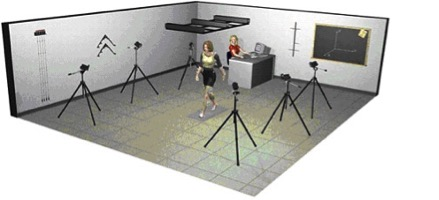
\includegraphics[width=0.9\textwidth]{./graphics/camera}
		\caption{Sistema de medida mediante cámaras} \label{fig:camera}
	\end{figure}
	
	\subsection{Sistemas optoelectrónicos}
	
	Los sistemas optoelectrónicos captan señales luminosas de marcadores colocados en el cuerpo del sujeto a medir y las convierten en señales eléctricas (ver Figura \ref{fig:opt}). A pesar de que se trata de un completo y minucioso método de análisis de la marcha, no resulta muy práctico en el ámbito del análisis clínico. Al alto coste y complejidad del equipo hay que añadir el amplio espacio de trabajo necesario para mantener una línea de visión libre de obstáculos entre el sujeto y los sistemas de medida. Además, la complejidad y lentitud provocan que resulte tedioso el tomar varias medidas \cite{begona,opt}.
		\begin{figure}[H]
			\centering
			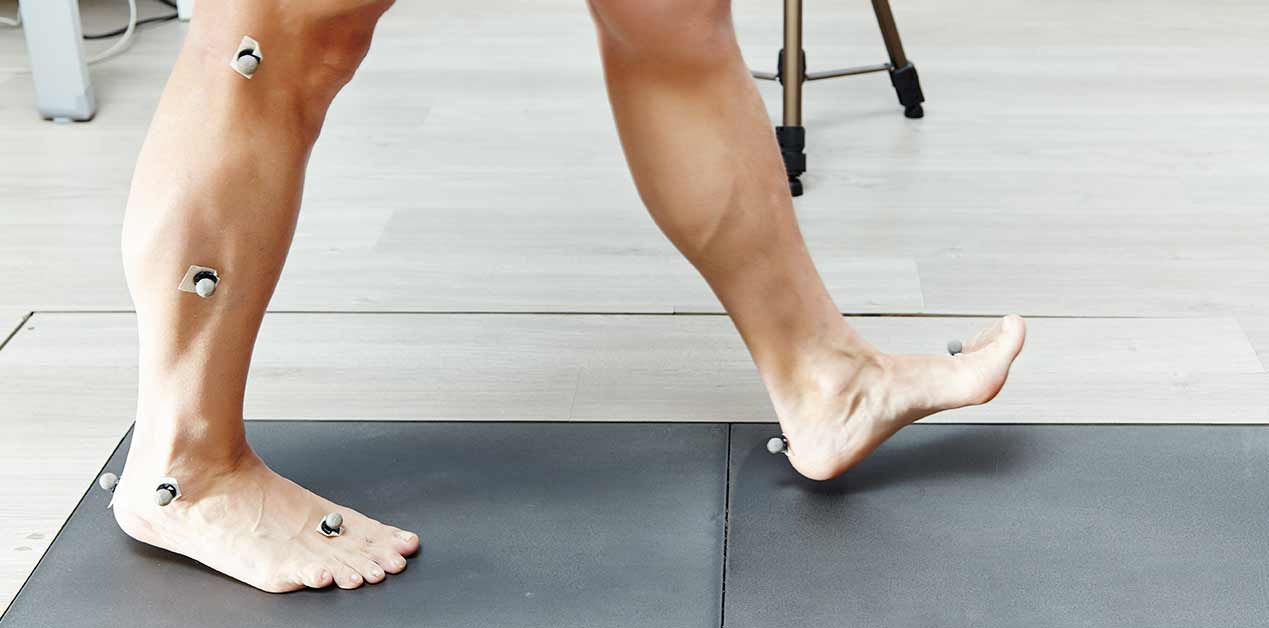
\includegraphics[width=0.9\textwidth]{./graphics/opt}
			\caption{Sistema de medida optoelectrónico} \label{fig:opt}
		\end{figure}

	\subsection{Tapices instrumentados}
	
	Existen sistemas como el GaitRite\textsuperscript{\textregistered} que permiten la medida de diferentes parámetros de la marcha, entre ellos la medida de distancia entre pasos \cite{gaitrite}. En la Figura \ref{fig:gaitrite} se observa dicho sistema el cual consiste en un tapiz instrumentado. Tiene como ventaja la portabilidad y la facilidad de manejo, así como el ahorro de tiempo debido a la automatización en el cálculo de los parámetros obtenidos. Sin embargo, existen ciertas limitaciones, dado que sólo se
	obtiene información de la presión ejercida sobre los sensores, sin tener en cuenta la
	dirección ni las componentes del vector de fuerza \cite{begona}. 
	
	\begin{figure}[H]
		\centering
		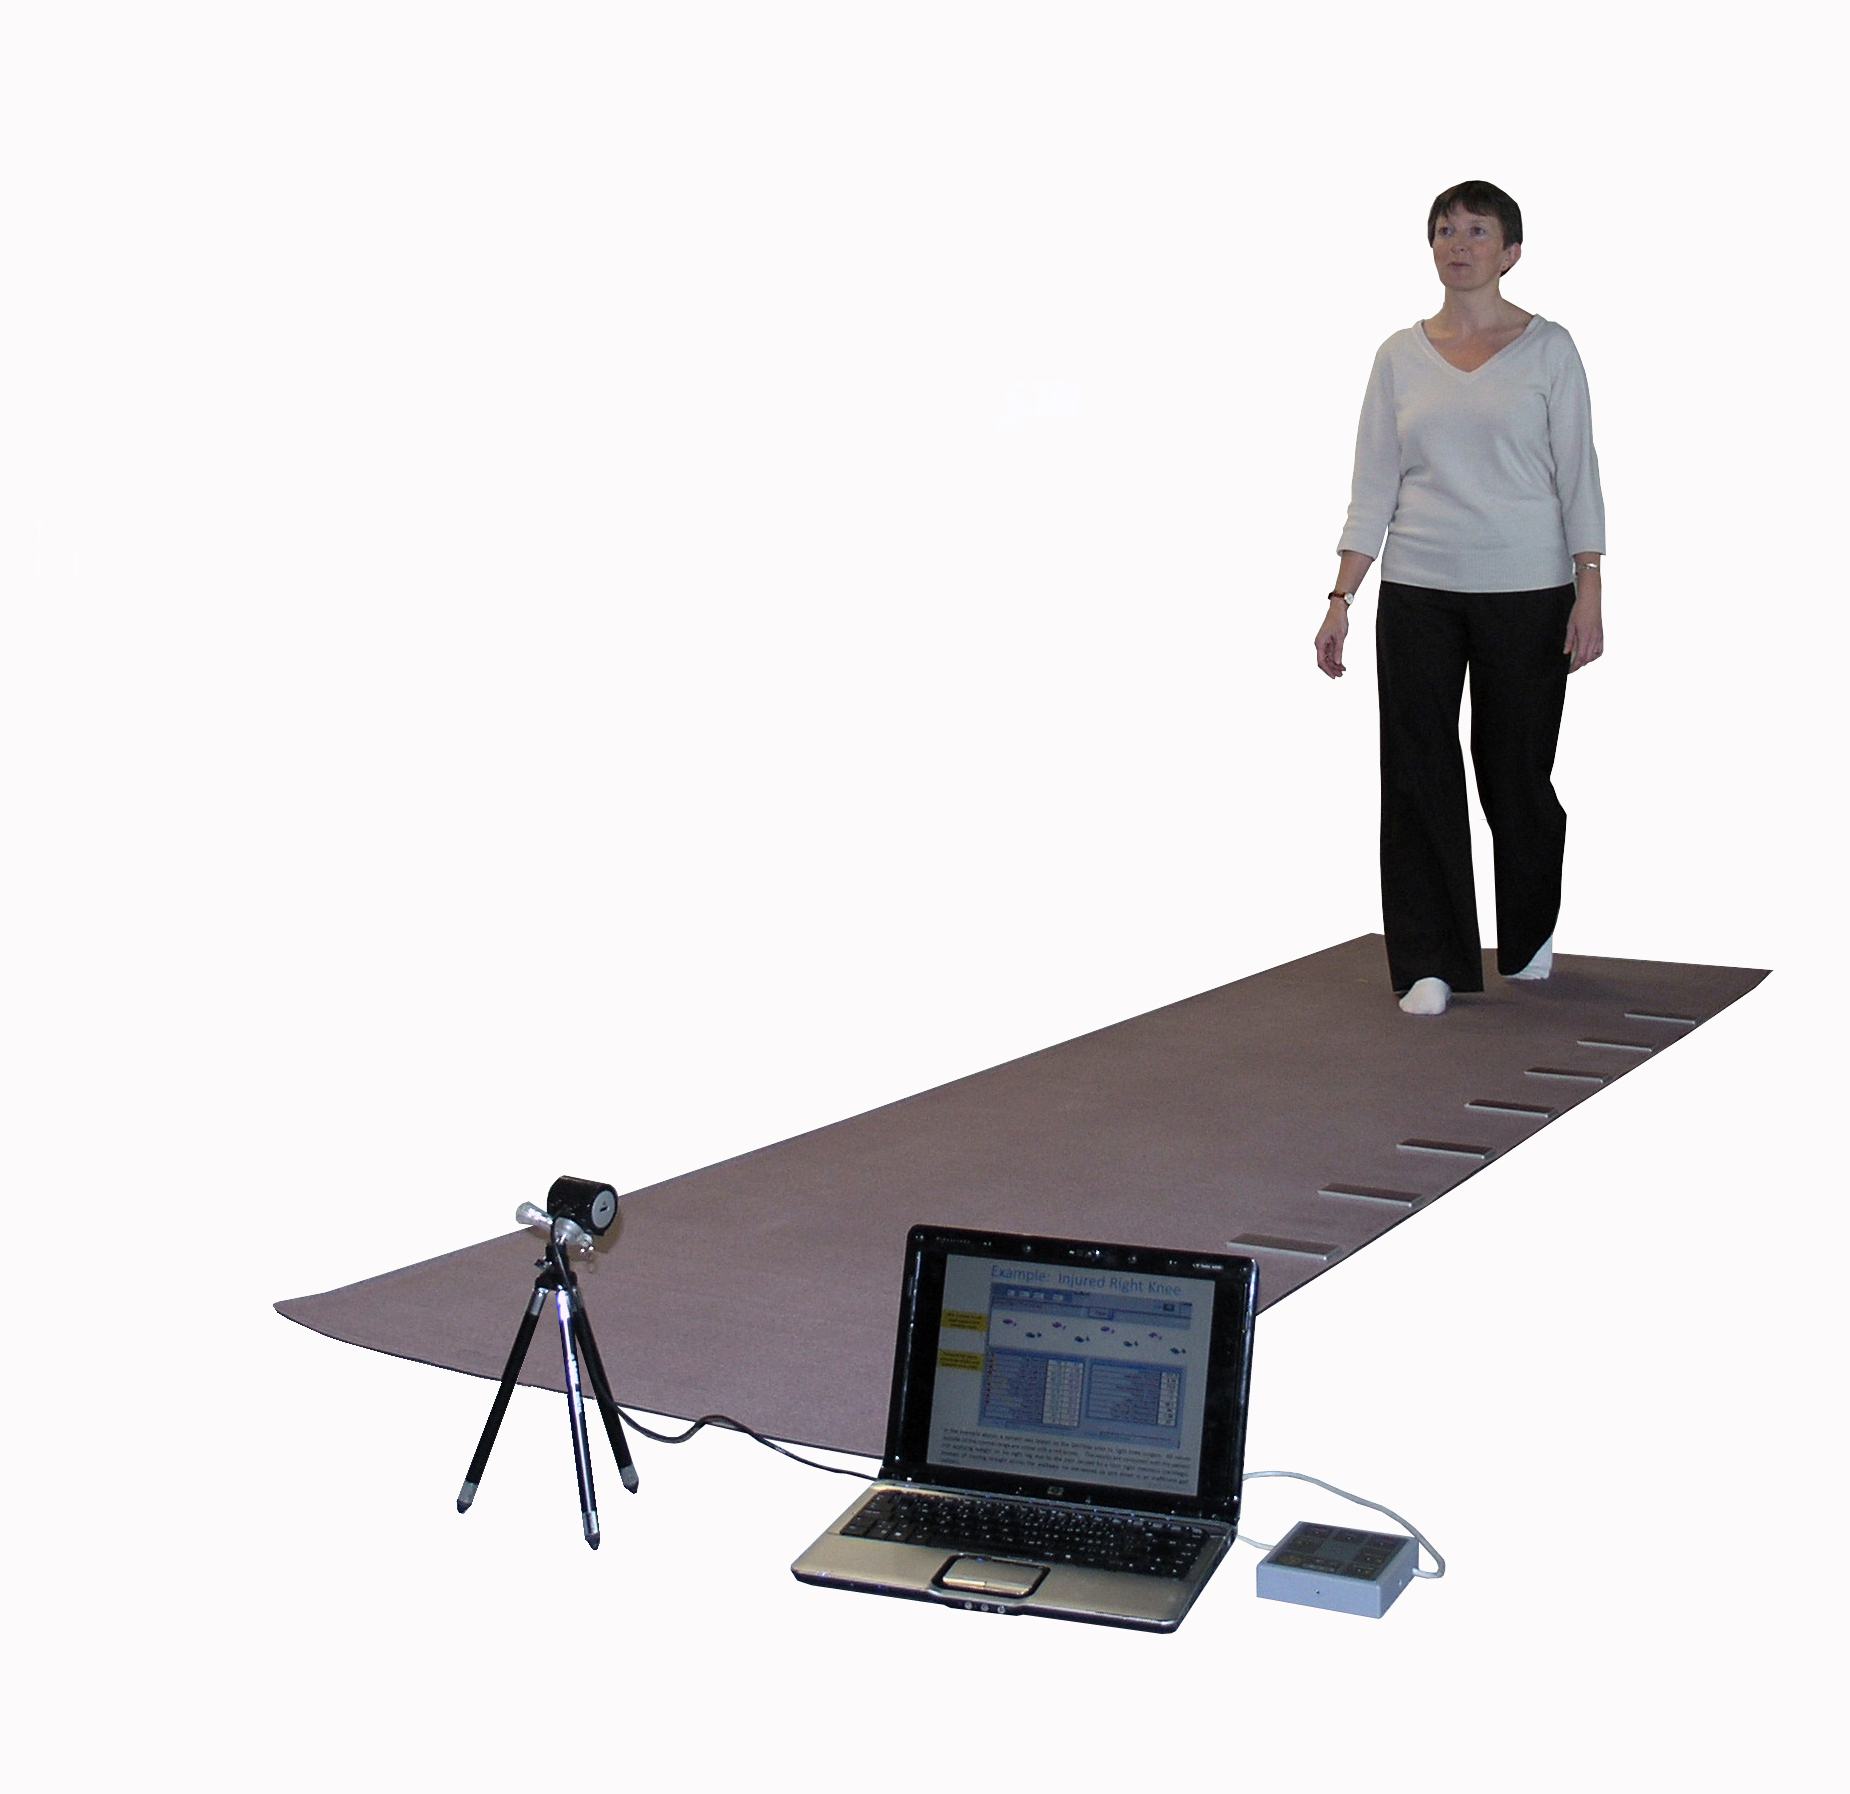
\includegraphics[width=0.6\textwidth]{./graphics/GaitRite}
		\caption{Sistema de medida GaitRite\textsuperscript{\textregistered}} \label{fig:gaitrite}
	\end{figure}
	
	\subsection{Zapatos instrumentados}
	
	\cite{shoes} Existe un sistema de medida integrado en zapatos que combina la utilización de sensores inerciales así como sensores de fuerza que completan la medida de los parámetros de la marcha. Se trata de un diseño compacto y que puede ser utilizado en entornos diferentes. En la Figura \ref{fig:shoes} aparece representado el diseño del zapato utilizado.
	
		\begin{figure}[H]
			\centering
			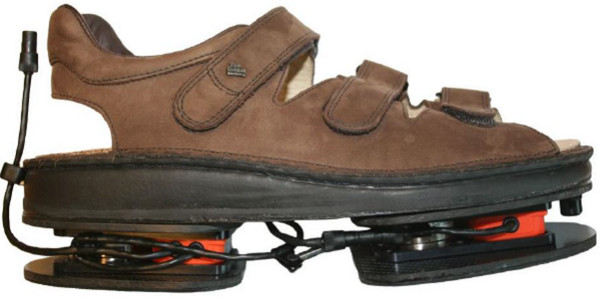
\includegraphics[width=0.6\textwidth]{./graphics/shoes}
			\caption{Zapatos instrumentados} \label{fig:shoes}
		\end{figure}
		 

Cada uno de los zapatos tienen un peso de aproximadamente 1.1Kg por lo que pueden afectar en la marcha a los pacientes ya que existe gran probabilidad de que hayan perdido fuerza en alguno de los lados. Además, únicamente con estos zapatos no es posible el cálculo de la distancia entre pasos por lo que aparecen nuevas versiones en las que se añaden sensores de ultrasonidos y por tanto reducen la ergonomía del sistema  \cite{shoes} . 


	
	
	